\documentclass[12pt,A4paper,oneside]{amsart}

%\usepackage{color,graphicx}
%\usepackage{mathrsfs,amsbsy}
\usepackage{bm}
\usepackage{booktabs}
\usepackage{ctex}
\usepackage{amssymb}
\usepackage{amsmath}
\usepackage{amsfonts}
\usepackage{array}
\usepackage{fancyhdr}
\usepackage{hhline}
\usepackage[unicode, bookmarksnumbered]{hyperref}	% 启动超链接和 PDF 文档信息所需
\usepackage{graphicx}
\usepackage{amsthm}
\usepackage{enumerate}
\usepackage[mathscr]{eucal}
\usepackage{mathrsfs}
\usepackage{verbatim}
\usepackage{wrapfig}
\usepackage{geometry} %调整页面的页边距
\usepackage{pifont}
\geometry{left=2.5cm,right=2.5cm,top=2cm,bottom=2.5cm}%具体的页边距设置
%\usepackage[notcite,notref]{showkeys}

% showkeys  make label explicit on the paper

%\makeatletter
%\@namedef{subjclassname@2010}{%
%  \textup{2010} Mathematics Subject Classification}
%\makeatother

\numberwithin{equation}{section}

\theoremstyle{plain}
\newtheorem{theorem}{Theorem}[section]
\newtheorem{lemma}[theorem]{Lemma}
\newtheorem{proposition}[theorem]{Proposition}
\newtheorem{corollary}[theorem]{Corollary}
\newtheorem{claim}[theorem]{Claim}
\newtheorem{defn}[theorem]{Definition}
\newtheorem{example}[theorem]{Example}

\theoremstyle{plain}
\newtheorem{exercise}{Exercise}[section]

\theoremstyle{plain}
\newtheorem{thmsub}{Theorem}[subsection]
\newtheorem{lemmasub}[thmsub]{Lemma}
\newtheorem{corollarysub}[thmsub]{Corollary}
\newtheorem{propositionsub}[thmsub]{Proposition}
\newtheorem{defnsub}[thmsub]{Definition}

\numberwithin{equation}{section}


\theoremstyle{remark}
\newtheorem{remark}[theorem]{Remark}
\newtheorem{remarks}{Remarks}

\newcommand*{\thick}[1]{\text{\boldmath$#1$}}
\newcommand*{\cir}[1]{\;$\ding{19#1}$\;}%临时使用
\newcommand*{\norm}[1]{\lVert#1\rVert}

%\renewcommand\thefootnote{\fnsymbol{footnote}}
%dont use number as footnote symbol, use this command to change

\DeclareMathOperator{\supp}{supp}
\DeclareMathOperator{\dist}{dist}
\DeclareMathOperator{\vol}{vol}
\DeclareMathOperator{\diag}{diag}
\DeclareMathOperator{\tr}{tr}


\begin{document}

\title[]{\LARGE $\mathbb{R}^n$中的拓扑}


\author[]{\large 周潇翔}
\address{School of Mathematical Sciences\\
University of Science and Technology of China\\
Hefei, 230026\\ P.R. China\\}
\email{xx352229@mail.ustc.edu.cn}
\maketitle




\begin{abstract}
介绍一个我大一时为了理解$\mathbb{R}^n$中的拓扑概念而使用的一套方法,这种方法也可以推广至一般的度量空间的情况,不过还是在$\mathbb{R}^n$中,尤其是\protect{$\mathbb{R}$}中显得最清楚.这种方法对我开始时厘清概念起到相当大的帮助,但之后便不会再用到,所以可以将其视为“拓扑初级阶段”.
\end{abstract}




%%%%%%%%%%%%%%%%%%%%%%%%%%%%%%%%%%%%%%%%%%%%%%%%%%%%%%%%%%%%%%%%%%%%%%%%%%%%%%%%%%%%%%%%%%%%%

在拓扑学中,我们往往会对一个集合的子集感兴趣.自然地,在$\mathbb{R}^n$中,我们会对$\mathbb{R}^n$的子集感兴趣.我们会如何来利用这个给定的集合,分析它的性质呢?

\begin{example}\label{ex1}
	观察集合$E:\{(x,y) \in \mathbb{R}^2\mid y\geqslant x^2\}$可以直观地感觉到$\mathbb{R}^2$被这个集合分成了3个部分:
\begin{figure}[ht]
	\begin{minipage}[b]{.60\textwidth}

			\begin{itemize}
				\item $E$的内部$E^{\circ}=\{(x,y) \in \mathbb{R}^2\mid y> x^2\}$
				\item $E$的边界$\partial E=\{(x,y) \in \mathbb{R}^2\mid y= x^2\}$
				\item $E$的外部$(E^c)^{\circ}=\{(x,y) \in \mathbb{R}^2\mid y< x^2\}$
			\end{itemize}	
当然,我们自然留下了许多无法解决的问题.什么是$E$的内部、边界和外部?为何我们就能将其恰好分成这三个部分?为此,我们需要剖析我们自己的直觉:我们是如何通过自己的直觉来辨别出这些元素的不同的?如何将我们的这一点直观转换成严谨的数学语言?
	\end{minipage}
	\begin{minipage}[b]{.38\textwidth}
		\centering
		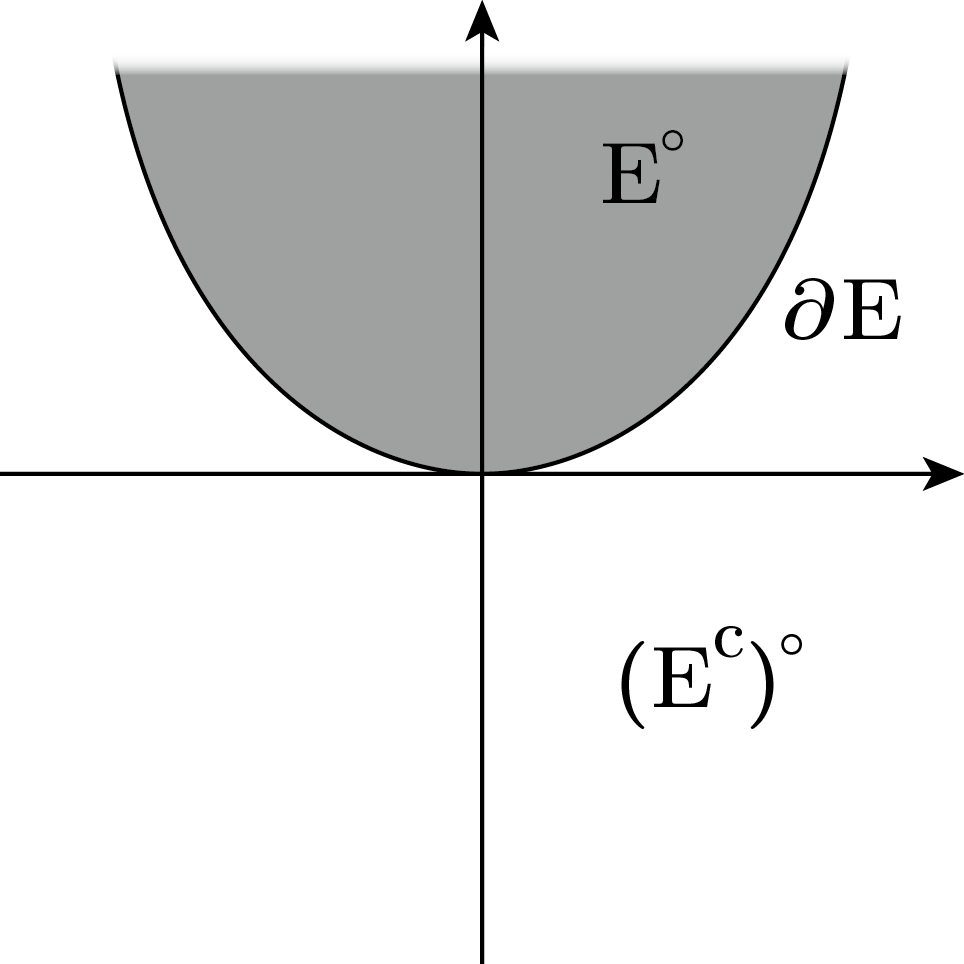
\includegraphics[width=4cm]{figures/figure2.png}
		\caption{$E$}
	\end{minipage}

\end{figure}	
\end{example}
\section{$E$对$\mathbb{R}^n$的分类}
在这里,我们想用集合$E \subseteq \mathbb{R}^n$来将$\mathbb{R}^n$分成几块.有一个标准是既简单又直接的:按照点在不在集合$E$中,先将$\mathbb{R}^n$分成两大块:$\mathbb{R}^n=E \sqcup E^c$\footnote{这里$\sqcup$表示无交并的意思,有两层意义:1.(表并)$\mathbb{R}^n=E \cup E^c$;$\qquad$2.(无交)$E \cap E^c = \varnothing$.}

\begin{exercise}
	\label{exer:cantorset}
	试从网上查阅Cantor集$\mathcal{C}$的定义,将集合$$A=\left\{\frac{p}{q}\;\bigg| p,q \in \mathbb{Z}, 0 < p \leqslant q \leqslant 5 \right\}$$按照是否落在$\mathcal{C}$中分为两类.
\end{exercise}
\begin{figure}[th]
	\centering
	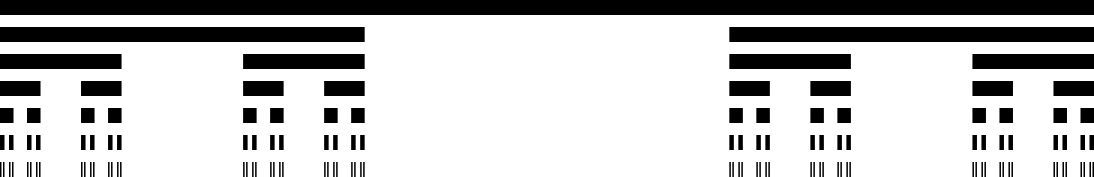
\includegraphics[width=\textwidth]{figures/Cantor_set.jpg}\\
	\caption{生成Cantor集的最初几步}
\end{figure}
但这难以完全满足我们的需求.我们看到我们对$\mathbb{R}^n$中点的分类,不止关注这个点的情况,还在这个点附近的情况.故我们引入点的空心球(去心邻域)\footnote{实际的去心邻域的概念更广,不过我们也不涉及.}的概念:


	\begin{figure}[ht]
		\begin{minipage}[b]{.65\textwidth}
			\begin{defn}[空心球]
				我们称
			$$B_r(\check{\thick{a}})=\{\thick{x} \in \mathbb{R}^n \mid 0 < \norm{\thick{x}-\thick{a}} <r\}$$
			为以$\thick{a}$为球心,以$r>0$为半径的\bfseries{空心球(open ball of radius r around $\thick{a}$)}.
			\end{defn}
		\end{minipage}
		\begin{minipage}[b]{.33\textwidth}
			\centering
			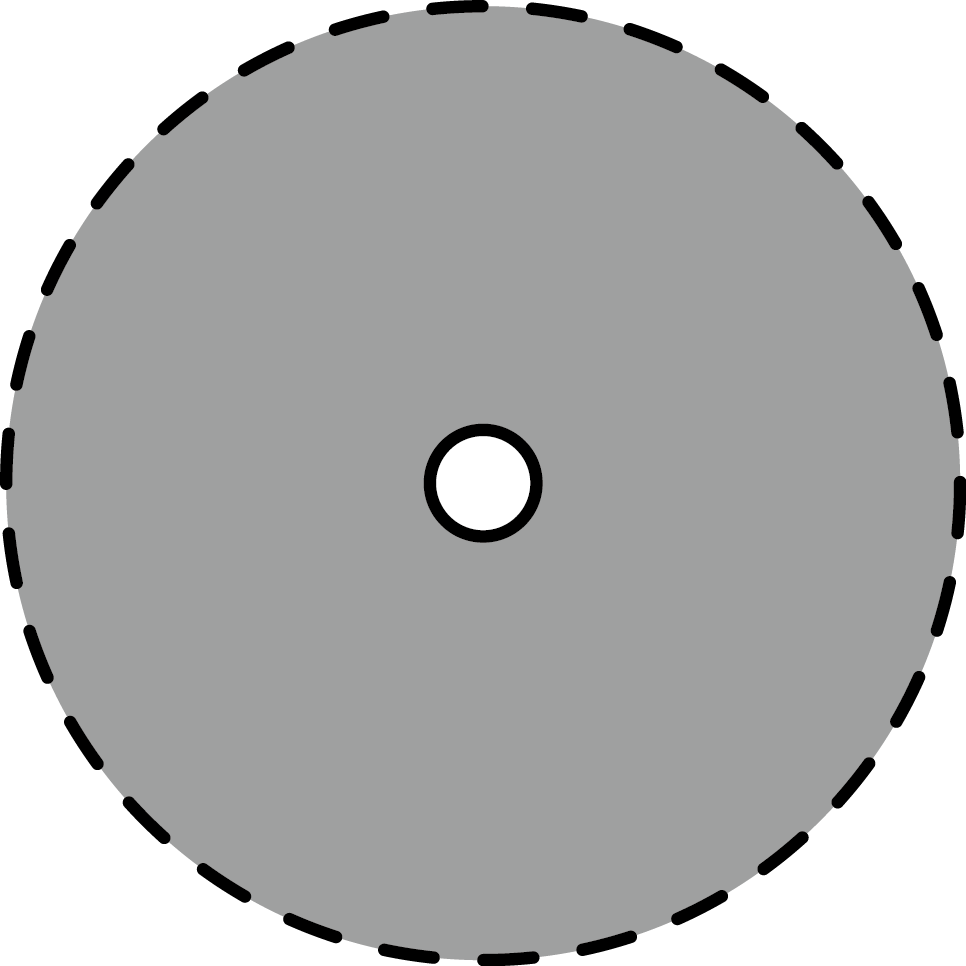
\includegraphics[width=2cm]{figures/figure3.png}
			\caption{空心球}
		\end{minipage}
		
	\end{figure}


事实上,一个足够小的空心球能够充分地体现一个点附近的情况.\footnote{我们之所以用空心球而不用球$B_r(\thick{a})$,是由于点$\thick{a}$过于特殊.}下面的定义是为了叙述方便使用,用过后可以直接忘却即可.

\begin{defn}[被$E$包围]
	我们称点$\thick{a}$被$E$包围,是指存在$r>0$,使得$B_r(\check{\thick{a}}) \subseteq E$\footnote{注意这里我们没有要求$\thick{a} \in E$或$\thick{a} \notin E$.}.
\end{defn}
\begin{corollary}
	点$\thick{a}$被$E^c$包围,当且仅当存在$r>0$,使得$B_r(\check{\thick{a}}) \subseteq E^c$
\end{corollary}
容易看出对于一个给定的点$\thick{a}$,这两种情况不会同时发生(作为练习).我们将其余的情况划为第三类,这样我们就成功地从另一种角度(点附近的情况)来将$\mathbb{R}^n$中的点集分类.
\begin{exercise}
	按照被$E$包围、被$E^c$包围和其他情况将\textbf{Example \ref{ex1}} 中的$\mathbb{R}^2$分为三类.
\end{exercise}
在介绍开集闭集这些概念之前,我们先来深入探讨下“被$E$包围”相关的等价叙述.
\begin{defn}[聚点\footnote{见\cite[p325,定义8.3.3]{CS12}.}]
	我们称$a$为$E$的\textbf{聚点(accumulated point)}(凝聚点,极限点),如果对任意$r>0$,总存在$x \in E$,使得$x \in B_r(\check{\thick{a}})$.
\end{defn}
聚点有许多等价的定义,兹列举如下:
\begin{equation*}
\begin{aligned}
\text{$\thick{a}$为$E$的聚点}&\Leftrightarrow \text{对任意$r>0,$总存在$x \in E,$使得$x \in B_r(\check{\thick{a}})$}\\
&\Leftrightarrow \text{对任意$r>0, B_r(\check{\thick{a}}) \cap E \neq \varnothing$}\\
&\Leftrightarrow \text{存在不取值于$\thick{a}$的数列$\{a_n\} \subseteq E$收敛于$\thick{a}$}\\
&\Leftrightarrow \text{存在数列$\{a_n\} \subseteq E$收敛于$\thick{a}$,且对任意$n \neq m,$有$a_n \neq a_m$}
\end{aligned}
\end{equation*}
下面的性质和推论是自然的,留作习题.
\begin{proposition}\
	\begin{itemize}
		\item 点$\thick{a}$不被$E$包围$\Longleftrightarrow$点$\thick{a}$为$E^c$的聚点
		\item 点$\thick{a}$不被$E^c$包围$\Longleftrightarrow$点$\thick{a}$为$E$的聚点
	\end{itemize}
\end{proposition}
\begin{corollary}
	点$\thick{a}$为第三类情况$\Longleftrightarrow$点$\thick{a}$同时为$E$与$E^c$的聚点,i.e.在$E\smallsetminus\{\thick{a}\}$中存在收敛于$\thick{a}$的数列,且在$E^c\smallsetminus\{\thick{a}\}$中存在收敛于$\thick{a}$的数列.
\end{corollary}
这时候我们可以说是相当清晰地描述了一个点附近的三种情况.将点与点附近的情况组合起来考虑,我们得到了一个对全集$\mathbb{R}^n$的分划:

\begin{table}[ht]
	\centering
\renewcommand\arraystretch{2}
%\begin{tabular}{|c||c|c|c|}
%	\hline
%	& 被$E$包围 & 其它 & 被$E^c$包围 \\ 
%	\hhline {|=::=:=:=|}
%	$\thick{a} \in E$	&$\partial E$
%	&\ding{193}  &\ding{194}  \\ 
%	\hline 
%	$\thick{a} \notin E$	&\ding{195}  &\ding{196}  &\ding{197}  \\ 
%	\hline
%\end{tabular} \\[0.5cm]
    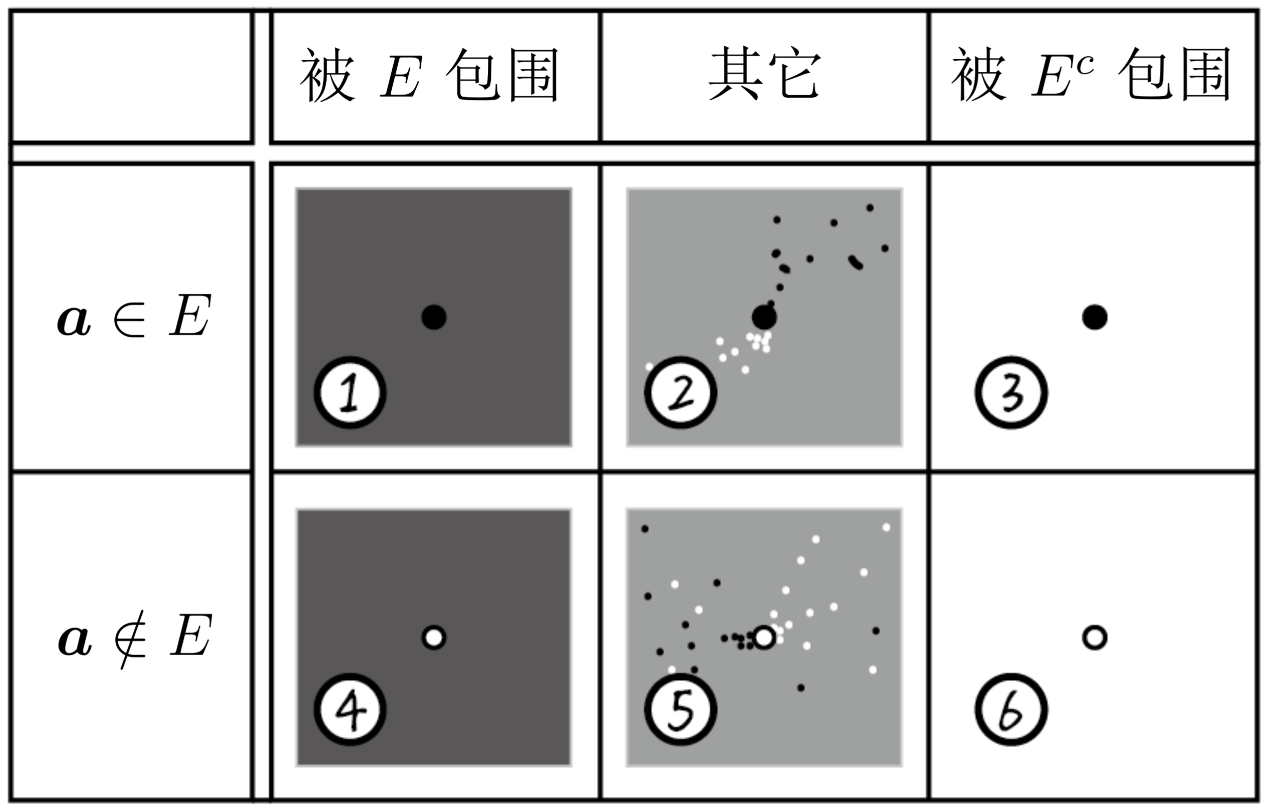
\includegraphics[width=.5\textwidth]{figures/bigtable.png}\\
	\caption{对$\mathbb{R}^n$彻底的分类}
	\label{bigtable1}
\end{table}

\begin{exercise}
	\label{exer:classify}
	指出在\textbf{Example \ref{ex1}}中的\ding{192}$\sim$\ding{197}.哪几部分为空集?\\
	当$n=1,E=\mathcal{C}$时,指出\ding{192}$\sim$\ding{197}.哪几部分为空集?在\textbf{Exercise \ref{exer:cantorset}}中,集合$A$中的元素各在哪个位置?
\end{exercise}


\section{开集与闭集}
我们来利用我们的分类来研究开集和闭集.
\begin{defn}[内点,内部\footnote{见\cite[p322,定义8.3.1]{CS12}.}]
	设$E \subseteq \mathbb{R}^n$.如果点$\thick{a} \in E$,并且存在$r>0$,使得$B_r(\thick{a}) \subseteq E$,那么称$\thick{a}$为$E$的一个\textbf{内点(interior point)}.点集$E$的全体内点所构成的集合记作$E^{\circ}$,称之为$E$的\textbf{内部(interior)}.\footnote{注意元素与集合的区别.内点是$E$的元素,而内部为$E$的子集.}
\end{defn}
来观察我们的分划.$E$的内点按照定义,首先落在$E$中,然后又被$E$包围,故一定落在\ding{192}中.反过来,落在\ding{192}中的元素一定为$E$的内点.\footnote{不过是同义反复.}故集合$E$的内部恰好即为\ding{192}.
\renewcommand\arraystretch{2}
\begin{table}[ht]
\begin{minipage}[t]{.48\textwidth}
	\centering
\begin{tabular}{>{\centering\arraybackslash}p{1cm}*{2}{|>{\centering\arraybackslash}p{1cm}}}
	\centering	$\checkmark$	&  &  \\\hline 
	&  &  \\ 
\end{tabular} \\[0.5cm]
	\caption{内点与内部}
	\label{table1}
\end{minipage}
\begin{minipage}[t]{.48\textwidth}
	\centering
	\begin{tabular}{>{\centering\arraybackslash}p{1cm}*{2}{|>{\centering\arraybackslash}p{1cm}}}
		& $\times$ & $\times$ \\\hline
		&  &  \\
	\end{tabular} \\[0.5cm]
	\caption{开集}
	\label{table2}
\end{minipage}
\end{table}
\begin{defn}[开集与闭集]
	我们称$E$为$\mathbb{R}^n$的\textbf{开集(open set)},若$E=E^{\circ}$.如果$E^c$为开集,则称$E$为闭集.
\end{defn}
观察到$E=\cir{2}\sqcup\cir{3}\sqcup\cir{4}$而$E^{\circ}=\cir{2}$,故$E$为开集$\Longleftrightarrow \cir{3}=\cir{4}=\varnothing$.
为了更好地了解闭集的信息,我们想知道$E$与$E^c$将集合分成的六类中有没有什么相关性.很明显是有的:
\begin{table}[ht]
	\begin{minipage}[t]{.48\textwidth}
		\centering
		\renewcommand\arraystretch{1}
		\begin{tabular}{|c||c|c|c|}
			\hline
			& 被$E^c$包围 & 其它 & 被$(E^c)^c$包围 \\ 
			\hhline {|=::=:=:=|}
			$\thick{a} \in E^c$	&\ding{197} &\ding{196}  &\ding{195}  \\ 
			\hline 
			$\thick{a} \notin E^c$	&\ding{194}  &\ding{193}  &\ding{192}  \\ 
			\hline
		\end{tabular}\\[0.65cm]
		\caption{$E^c$分成的6类}
		\label{table3}
	\end{minipage}
	\begin{minipage}[t]{.48\textwidth}
		\centering
		\renewcommand\arraystretch{2}
		\begin{tabular}{>{\centering\arraybackslash}p{1cm}*{2}{|>{\centering\arraybackslash}p{1cm}}}
			&  &  \\\hline
			$\times$ & $\times$ &  \\
		\end{tabular} \\[0.5cm]
		\caption{闭集}
		\label{table4}
	\end{minipage}
\end{table}
故$E$为闭集$\Longleftrightarrow E^c$为开集$\Longleftrightarrow \cir{5}=\cir{6}=\varnothing$.
\begin{exercise}
	由\textbf{Exercise \ref{exer:classify}},直接说明\textbf{Example \ref{ex1}}中的$E$与Cantor集分别为$\mathbb{R}^2$与$\mathbb{R}$中的闭集.
\end{exercise}
\cite[p325,推论8.3.1]{CS12}是关于闭集的等价定义,这个定义对于理解``$\mathbb{R}^n$中,列紧集$\Leftrightarrow$有界闭集"非常有帮助,且这个定义在泛函分析中被多次使用(其对一般的度量空间也是成立的).

我们来开始肝这一节中最难的几个定义.在这之前,我们回顾下聚点这个概念:\\
点$\thick{a}$为$E$的聚点$\Longleftrightarrow$点$\thick{a}$不被$E^c$包围$\Longleftrightarrow \thick{a} \notin \cir{4} \sqcup \cir{7} \Longleftrightarrow \thick{a} \in \cir{2} \sqcup \cir{3} \sqcup \cir{5} \sqcup \cir{6}$.\\
我们称$E$的全体凝聚点$E'$为$E$的\textbf{导集(derived set)},故$E'= \cir{2} \sqcup \cir{3} \sqcup \cir{5} \sqcup \cir{6}$
\begin{defn}[孤立点]
	我们称$\thick{a} \in E$为$E$的\textbf{孤立点(isolated point)},若$\thick{a}$不为聚点.
\end{defn}
\begin{exercise}
	验证$\thick{a}$为孤立点$\Longleftrightarrow \thick{a} \in \cir{4}$.
\end{exercise}
\begin{table}[ht]
	\begin{minipage}[t]{.32\textwidth}
		\centering
		\begin{tabular}{>{\centering\arraybackslash}p{1cm}*{2}{|>{\centering\arraybackslash}p{1cm}}}
		$\checkmark$	& $\checkmark$ &  \\\hline 
		$\checkmark$	& $\checkmark$ &  \\ 
		\end{tabular} \\[0.5cm]
		\caption{导集}
		\label{table5}
	\end{minipage}
	\begin{minipage}[t]{.32\textwidth}
		\centering
		\begin{tabular}{>{\centering\arraybackslash}p{1cm}*{2}{|>{\centering\arraybackslash}p{1cm}}}
			&  & $\checkmark$ \\\hline
			&  &  \\
		\end{tabular} \\[0.5cm]
		\caption{孤立点}
		\label{table6}
	\end{minipage}
	\begin{minipage}[t]{.32\textwidth}
		\centering
		\begin{tabular}{>{\centering\arraybackslash}p{1cm}*{2}{|>{\centering\arraybackslash}p{1cm}}}
		$\checkmark$	& $\checkmark$ & $\checkmark$ \\\hline 
		$\checkmark$	& $\checkmark$ &  \\ 
		\end{tabular} \\[0.5cm]
		\caption{闭包}
		\label{table7}
	\end{minipage}
\end{table}
\begin{exercise}
	定义$E$的\textbf{闭包(closure)}$\overline{E}=E \cup E'$.验证$\overline{E}=\cir{2} \sqcup \cir{3} \sqcup \cir{4} \sqcup \cir{5} \sqcup \cir{6}=\mathbb{R}^n \smallsetminus \cir{7}$,故而有推论$\overline{E}=((E^c)^{\circ})^c$.
\end{exercise}
接下来我就偷个懒,毕竟还是要留下自己思考的余地呀.
\begin{exercise}
	自行阅读\cite[p326,定义8.3.5]{CS12},利用分类的方法理解概念:外点与\textbf{外部 (exterior)};边界点与\textbf{边界 (boundary)}.画出表格(可参考表\ref{table1})并顺手证明$$E^{\circ} \sqcup (E^c)^{\circ} \sqcup \partial E = \mathbb{R}^n.$$
\end{exercise}
\begin{exercise}
	利用分类的方法刷完\cite[p327-328,练习题8.3]{CS12}的1-3,5,6,13.
\end{exercise}
\begin{exercise}\footnote{定义对称差(symmetric difference):$A \triangle B=(A \cap B^c) \sqcup (A^c \cap B)$.}
	考虑$\mathbb{R}^2$中的两个集合:$\mathcal{C} \times \mathcal{C}$与
	\begin{figure}[h]
		\centering
		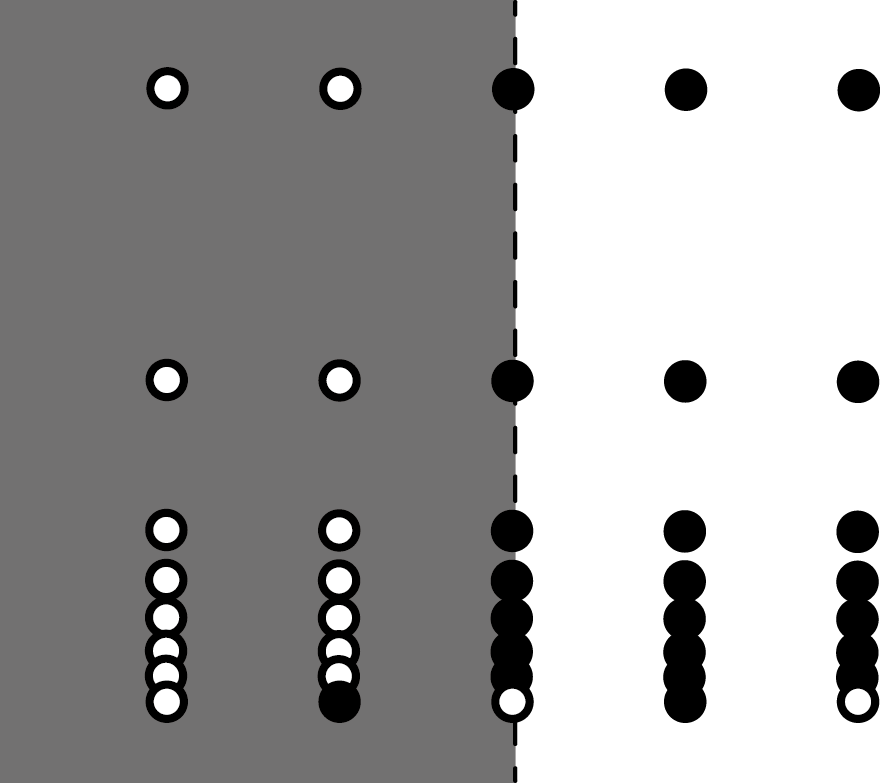
\includegraphics[width=4cm]{figures/figure4.png}\\[-0.5cm]
	\end{figure}
	$$\left((-\infty ,0)\times\mathbb{R}\right)\triangle \left( \{-2,-1,0,1,2\}\times \{0\} \bigcup \{-1,1\} \times \left\{\frac{1}{n}\Bigg{|} n \in \mathbb{N}^+ \right\}\right)$$
	它们是开集、闭集、有界集吗?它们的导集、闭包、内部、外部、边界分别是什么?有无孤立点?
\end{exercise}
\begin{exercise}
	定义$$A_n=\{(0.j_1j_2\cdots j_n)_3 \mid j_i=0 ,2 \text { for } i \in \{1,2, \ldots,n\}\}\qquad A=\bigcup_{n=1}^{+\infty} A_n$$
	说明$\mathcal{C}\neq A$而$\mathcal{C} = \overline{A}$.(许多人问Cantor集是不是就是边界点集的并,这个练习可以说明这一点是错误的,但是``很接近":Cantor集是边界点集的并的闭包.)
\end{exercise}
\section{后记}
这份材料与其说是介绍$\mathbb{R}^n$中的拓扑,不如说是对教材\cite[8.3]{CS12}中内容的一个导读.我希望这份材料能使同学克服阅读\cite[8.3]{CS12}的一些障碍,并获得阅读材料\cite[Appendix A]{JM08}的能力.

还有许多的内容我没有提到,索性在这里一并提一提.
\begin{itemize}
	\item 定理8.3.6是很有意思的一个定理,它说明了内部与闭包的特殊性.(你也可以说这两个概念是对偶的).
	\item 定理8.3.3以后会推广到抽象的拓扑空间中作为开集的定义.
	\item \cite[8.4]{CS12}主要就是定义(列紧集和紧集(紧致集))与一个结论$\mathbb{R}^n$中有界闭集$\Leftrightarrow$紧集$\Leftrightarrow$列紧集,证明是很漂亮的,结论也很重要(例如,你就可以说明有界闭集上的连续函数一定取到最值了).
	\item \cite[8.5]{CS12}主要和连通性有关,看之前可以想想如果是自己的话,会怎样定义一个集合的连通性.亦有一些非平凡的有趣的结论.比如,为什么$\mathbb{R}^n$中又开又闭的集合只有$\mathbb{R}^n$和$\varnothing$?
\end{itemize}
另外,这里术语的英文翻译主要参照\cite[Appendix A]{JM08}.还有借了下wiki的图片.
%%%%%%%%%%%%%%%%%%%%%%%%%%%%%%%%%%%%%%%%%%%%%%%%%%%%%%%%%%%%%%%%%%%%%%%%%%%%%%%%%%%%%%%%%%%%%





%%%%%%%%%%%%%%%%%%%%%%%%%%%%%%%%%%%%%%%%%%%%%%%%%%%%%%%%%%%%%%%%%%%%%%%%%%






%%%%%%%%%%%%%%%%%%%%%%%%%%%%%%%%%%%%%%%%%%%%%%%%%%%%%%%%%%%%%%%%%%%%%%%%%%%%%%%%%%%%%%%%%%%%%%%




\begin{thebibliography}{99}


%\bibitem{AF12}%
%Antunes, P., Freitas, P.: Optimal spectral rectangles and lattice ellipses. \emph{Proc. Royal Soc. London Ser. A.} \textbf{469} (2012), 20120492.
\bibitem{CS12}%
常庚哲,史济怀. 数学分析教程(第3版). 合肥:中国科学技术大学出版社,2012.8.
\bibitem{JM08}%
Lee J M. \emph{Introduction to smooth manifolds[M]}. 2008.
\bibitem{MAA97}
Armstrong M A. \emph{Basic topology[J]}. Undergraduate Texts in Mathematics, 1997:137-155.
\bibitem{JM00}
James Munkres. \emph{Topology}. 2nd. Prentice-Hall, Inc., Jan. 2000. ISBN: 9788120320468
\bibitem{YCY97}%
尤承业,《基础拓扑学讲义》,北京大学出版社,1997
\bibitem{XJC81}%
熊金城,《点集拓扑讲义》,人民教育出版社,1981
\bibitem{ZZM99}%
伏·巴尔佳斯基,伏·叶弗来莫维契,裘光明. 拓扑学奇趣[J].湖南教育出版社,1999.8.
\bibitem{AH03}%
Allen Hatcher. \emph{Algebraic topology}. Cambridge, New York: Cambridge University Press, 2003. isbn: 0-521-79160-X
\bibitem{EC18}
Evan Chen. \emph{An Infinitely Large Napkin}. draft. 2018.
URL:\href{http://web.evanchen.cc/napkin.html}{http://web.evanchen.cc/napkin.html}




\end{thebibliography}


\end{document}




